\documentclass[1p]{elsarticle_modified}
%\bibliographystyle{elsarticle-num}

%\usepackage[colorlinks]{hyperref}
%\usepackage{abbrmath_seonhwa} %\Abb, \Ascr, \Acal ,\Abf, \Afrak
\usepackage{amsfonts}
\usepackage{amssymb}
\usepackage{amsmath}
\usepackage{amsthm}
\usepackage{scalefnt}
\usepackage{amsbsy}
\usepackage{kotex}
\usepackage{caption}
\usepackage{subfig}
\usepackage{color}
\usepackage{graphicx}
\usepackage{xcolor} %% white, black, red, green, blue, cyan, magenta, yellow
\usepackage{float}
\usepackage{setspace}
\usepackage{hyperref}

\usepackage{tikz}
\usetikzlibrary{arrows}

\usepackage{multirow}
\usepackage{array} % fixed length table
\usepackage{hhline}

%%%%%%%%%%%%%%%%%%%%%
\makeatletter
\renewcommand*\env@matrix[1][\arraystretch]{%
	\edef\arraystretch{#1}%
	\hskip -\arraycolsep
	\let\@ifnextchar\new@ifnextchar
	\array{*\c@MaxMatrixCols c}}
\makeatother %https://tex.stackexchange.com/questions/14071/how-can-i-increase-the-line-spacing-in-a-matrix
%%%%%%%%%%%%%%%

\usepackage[normalem]{ulem}

\newcommand{\msout}[1]{\ifmmode\text{\sout{\ensuremath{#1}}}\else\sout{#1}\fi}
%SOURCE: \msout is \stkout macro in https://tex.stackexchange.com/questions/20609/strikeout-in-math-mode

\newcommand{\cancel}[1]{
	\ifmmode
	{\color{red}\msout{#1}}
	\else
	{\color{red}\sout{#1}}
	\fi
}

\newcommand{\add}[1]{
	{\color{blue}\uwave{#1}}
}

\newcommand{\replace}[2]{
	\ifmmode
	{\color{red}\msout{#1}}{\color{blue}\uwave{#2}}
	\else
	{\color{red}\sout{#1}}{\color{blue}\uwave{#2}}
	\fi
}

\newcommand{\Sol}{\mathcal{S}} %segment
\newcommand{\D}{D} %diagram
\newcommand{\A}{\mathcal{A}} %arc


%%%%%%%%%%%%%%%%%%%%%%%%%%%%%5 test

\def\sl{\operatorname{\textup{SL}}(2,\Cbb)}
\def\psl{\operatorname{\textup{PSL}}(2,\Cbb)}
\def\quan{\mkern 1mu \triangleright \mkern 1mu}

\theoremstyle{definition}
\newtheorem{thm}{Theorem}[section]
\newtheorem{prop}[thm]{Proposition}
\newtheorem{lem}[thm]{Lemma}
\newtheorem{ques}[thm]{Question}
\newtheorem{cor}[thm]{Corollary}
\newtheorem{defn}[thm]{Definition}
\newtheorem{exam}[thm]{Example}
\newtheorem{rmk}[thm]{Remark}
\newtheorem{alg}[thm]{Algorithm}

\newcommand{\I}{\sqrt{-1}}
\begin{document}

%\begin{frontmatter}
%
%\title{Boundary parabolic representations of knots up to 8 crossings}
%
%%% Group authors per affiliation:
%\author{Yunhi Cho} 
%\address{Department of Mathematics, University of Seoul, Seoul, Korea}
%\ead{yhcho@uos.ac.kr}
%
%
%\author{Seonhwa Kim} %\fnref{s_kim}}
%\address{Center for Geometry and Physics, Institute for Basic Science, Pohang, 37673, Korea}
%\ead{ryeona17@ibs.re.kr}
%
%\author{Hyuk Kim}
%\address{Department of Mathematical Sciences, Seoul National University, Seoul 08826, Korea}
%\ead{hyukkim@snu.ac.kr}
%
%\author{Seokbeom Yoon}
%\address{Department of Mathematical Sciences, Seoul National University, Seoul, 08826,  Korea}
%\ead{sbyoon15@snu.ac.kr}
%
%\begin{abstract}
%We find all boundary parabolic representation of knots up to 8 crossings.
%
%\end{abstract}
%\begin{keyword}
%    \MSC[2010] 57M25 
%\end{keyword}
%
%\end{frontmatter}

%\linenumbers
%\tableofcontents
%
\newcommand\colored[1]{\textcolor{white}{\rule[-0.35ex]{0.8em}{1.4ex}}\kern-0.8em\color{red} #1}%
%\newcommand\colored[1]{\textcolor{white}{ #1}\kern-2.17ex	\textcolor{white}{ #1}\kern-1.81ex	\textcolor{white}{ #1}\kern-2.15ex\color{red}#1	}

{\Large $\underline{12a_{0454}~(K12a_{0454})}$}

\setlength{\tabcolsep}{10pt}
\renewcommand{\arraystretch}{1.6}
\vspace{1cm}\begin{tabular}{m{100pt}>{\centering\arraybackslash}m{274pt}}
\multirow{5}{120pt}{
	\centering
	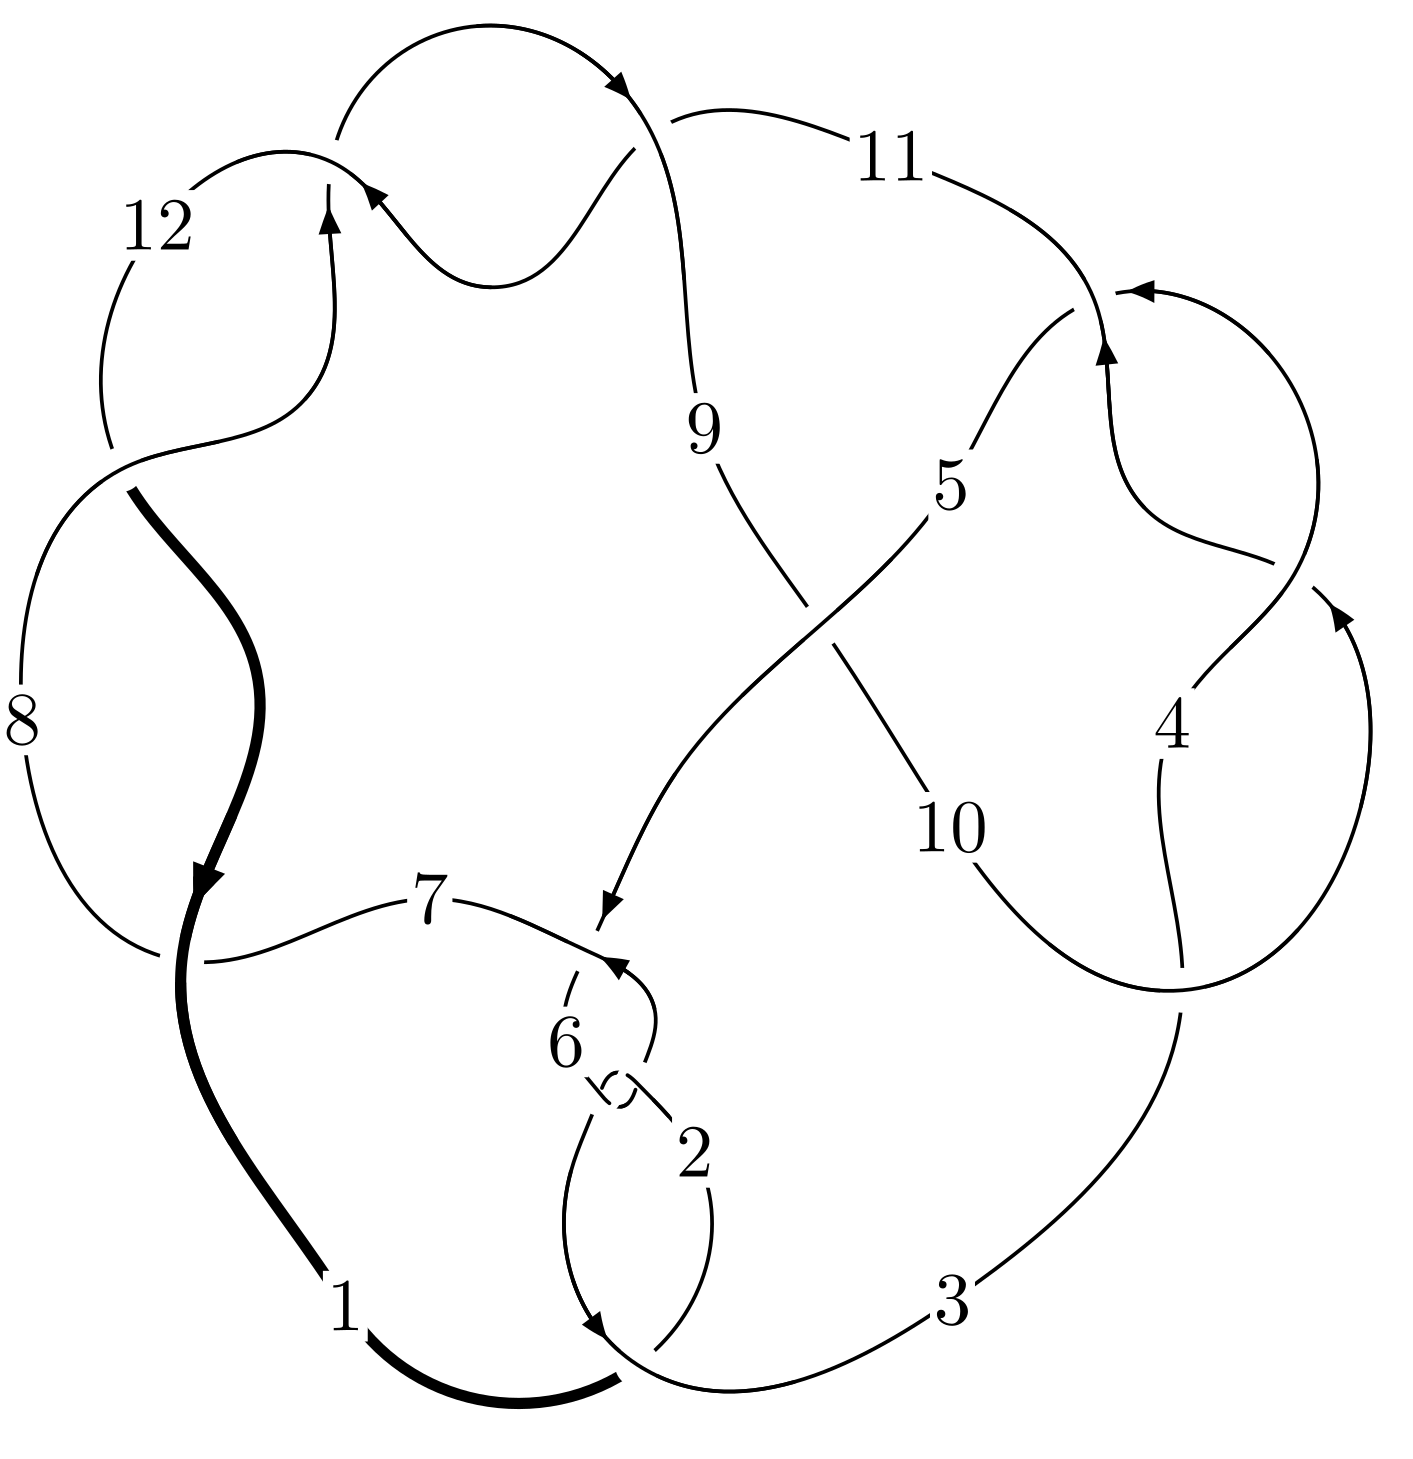
\includegraphics[width=112pt]{../../../GIT/diagram.site/Diagrams/png/1255_12a_0454.png}\\
\ \ \ A knot diagram\footnotemark}&
\allowdisplaybreaks
\textbf{Linearized knot diagam} \\
\cline{2-2}
 &
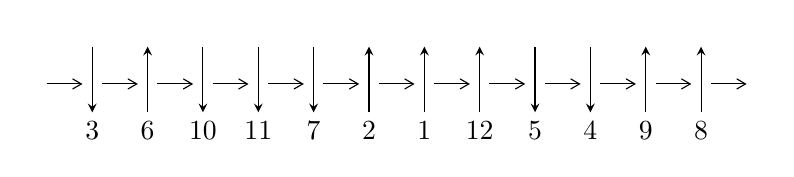
\begin{tikzpicture}[x=20pt, y=17pt]
	% nodes
	\node (C0) at (0, 0) {};
	\node (C1) at (1, 0) {};
	\node (C1U) at (1, +1) {};
	\node (C1D) at (1, -1) {3};

	\node (C2) at (2, 0) {};
	\node (C2U) at (2, +1) {};
	\node (C2D) at (2, -1) {6};

	\node (C3) at (3, 0) {};
	\node (C3U) at (3, +1) {};
	\node (C3D) at (3, -1) {10};

	\node (C4) at (4, 0) {};
	\node (C4U) at (4, +1) {};
	\node (C4D) at (4, -1) {11};

	\node (C5) at (5, 0) {};
	\node (C5U) at (5, +1) {};
	\node (C5D) at (5, -1) {7};

	\node (C6) at (6, 0) {};
	\node (C6U) at (6, +1) {};
	\node (C6D) at (6, -1) {2};

	\node (C7) at (7, 0) {};
	\node (C7U) at (7, +1) {};
	\node (C7D) at (7, -1) {1};

	\node (C8) at (8, 0) {};
	\node (C8U) at (8, +1) {};
	\node (C8D) at (8, -1) {12};

	\node (C9) at (9, 0) {};
	\node (C9U) at (9, +1) {};
	\node (C9D) at (9, -1) {5};

	\node (C10) at (10, 0) {};
	\node (C10U) at (10, +1) {};
	\node (C10D) at (10, -1) {4};

	\node (C11) at (11, 0) {};
	\node (C11U) at (11, +1) {};
	\node (C11D) at (11, -1) {9};

	\node (C12) at (12, 0) {};
	\node (C12U) at (12, +1) {};
	\node (C12D) at (12, -1) {8};
	\node (C13) at (13, 0) {};

	% arrows
	\draw[->,>={angle 60}]
	(C0) edge (C1) (C1) edge (C2) (C2) edge (C3) (C3) edge (C4) (C4) edge (C5) (C5) edge (C6) (C6) edge (C7) (C7) edge (C8) (C8) edge (C9) (C9) edge (C10) (C10) edge (C11) (C11) edge (C12) (C12) edge (C13) ;	\draw[->,>=stealth]
	(C1U) edge (C1D) (C2D) edge (C2U) (C3U) edge (C3D) (C4U) edge (C4D) (C5U) edge (C5D) (C6D) edge (C6U) (C7D) edge (C7U) (C8D) edge (C8U) (C9U) edge (C9D) (C10U) edge (C10D) (C11D) edge (C11U) (C12D) edge (C12U) ;
	\end{tikzpicture} \\
\hhline{~~} \\& 
\textbf{Solving Sequence} \\ \cline{2-2} 
 &
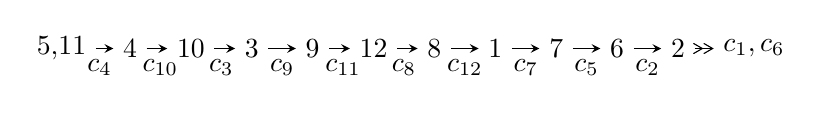
\begin{tikzpicture}[x=22pt, y=7pt]
	% node
	\node (A0) at (-1/8, 0) {5,11};
	\node (A1) at (1, 0) {4};
	\node (A2) at (2, 0) {10};
	\node (A3) at (3, 0) {3};
	\node (A4) at (4, 0) {9};
	\node (A5) at (5, 0) {12};
	\node (A6) at (6, 0) {8};
	\node (A7) at (7, 0) {1};
	\node (A8) at (8, 0) {7};
	\node (A9) at (9, 0) {6};
	\node (A10) at (10, 0) {2};
	\node (C1) at (1/2, -1) {$c_{4}$};
	\node (C2) at (3/2, -1) {$c_{10}$};
	\node (C3) at (5/2, -1) {$c_{3}$};
	\node (C4) at (7/2, -1) {$c_{9}$};
	\node (C5) at (9/2, -1) {$c_{11}$};
	\node (C6) at (11/2, -1) {$c_{8}$};
	\node (C7) at (13/2, -1) {$c_{12}$};
	\node (C8) at (15/2, -1) {$c_{7}$};
	\node (C9) at (17/2, -1) {$c_{5}$};
	\node (C10) at (19/2, -1) {$c_{2}$};
	\node (A11) at (45/4, 0) {$c_{1},c_{6}$};

	% edge
	\draw[->,>=stealth]	
	(A0) edge (A1) (A1) edge (A2) (A2) edge (A3) (A3) edge (A4) (A4) edge (A5) (A5) edge (A6) (A6) edge (A7) (A7) edge (A8) (A8) edge (A9) (A9) edge (A10) ;
	\draw[->>,>={angle 60}]	
	(A10) edge (A11);
\end{tikzpicture} \\ 

\end{tabular} \\

\footnotetext{
The image of knot diagram is generated by the software ``\textbf{Draw programme}" developed by Andrew Bartholomew(\url{http://www.layer8.co.uk/maths/draw/index.htm\#Running-draw}), where we modified some parts for our purpose(\url{https://github.com/CATsTAILs/LinksPainter}).
}\phantom \\ \newline 
\centering \textbf{Ideals for irreducible components\footnotemark of $X_{\text{par}}$} 
 
\begin{align*}
I^u_{1}&=\langle 
u^{51}- u^{50}+\cdots+2 u+1\rangle \\
\\
\end{align*}
\raggedright * 1 irreducible components of $\dim_{\mathbb{C}}=0$, with total 51 representations.\\
\footnotetext{All coefficients of polynomials are rational numbers. But the coefficients are sometimes approximated in decimal forms when there is not enough margin.}
\newpage
\renewcommand{\arraystretch}{1}
\centering \section*{I. $I^u_{1}= \langle u^{51}- u^{50}+\cdots+2 u+1 \rangle$}
\flushleft \textbf{(i) Arc colorings}\\
\begin{tabular}{m{7pt} m{180pt} m{7pt} m{180pt} }
\flushright $a_{5}=$&$\begin{pmatrix}1\\0\end{pmatrix}$ \\
\flushright $a_{11}=$&$\begin{pmatrix}0\\u\end{pmatrix}$ \\
\flushright $a_{4}=$&$\begin{pmatrix}1\\- u^2\end{pmatrix}$ \\
\flushright $a_{10}=$&$\begin{pmatrix}u\\- u^3+u\end{pmatrix}$ \\
\flushright $a_{3}=$&$\begin{pmatrix}- u^2+1\\u^4-2 u^2\end{pmatrix}$ \\
\flushright $a_{9}=$&$\begin{pmatrix}- u^3+2 u\\- u^3+u\end{pmatrix}$ \\
\flushright $a_{12}=$&$\begin{pmatrix}u^7-4 u^5+4 u^3\\u^7-3 u^5+2 u^3+u\end{pmatrix}$ \\
\flushright $a_{8}=$&$\begin{pmatrix}- u^{11}+6 u^9-12 u^7+8 u^5- u^3+2 u\\- u^{11}+5 u^9-8 u^7+3 u^5+u^3+u\end{pmatrix}$ \\
\flushright $a_{1}=$&$\begin{pmatrix}u^{15}-8 u^{13}+24 u^{11}-32 u^9+18 u^7-8 u^5+8 u^3\\u^{15}-7 u^{13}+18 u^{11}-19 u^9+6 u^7-2 u^5+4 u^3+u\end{pmatrix}$ \\
\flushright $a_{7}=$&$\begin{pmatrix}- u^{19}+10 u^{17}-40 u^{15}+80 u^{13}-83 u^{11}+50 u^9-36 u^7+24 u^5- u^3+2 u\\- u^{19}+9 u^{17}-32 u^{15}+55 u^{13}-45 u^{11}+19 u^9-16 u^7+10 u^5+3 u^3+u\end{pmatrix}$ \\
\flushright $a_{6}=$&$\begin{pmatrix}u^{38}-19 u^{36}+\cdots+2 u^2+1\\u^{38}-18 u^{36}+\cdots+6 u^4+u^2\end{pmatrix}$ \\
\flushright $a_{2}=$&$\begin{pmatrix}- u^{21}+10 u^{19}+\cdots+6 u^3- u\\u^{23}-11 u^{21}+\cdots+6 u^3+u\end{pmatrix}$\\&\end{tabular}
\flushleft \textbf{(ii) Obstruction class $= -1$}\\~\\
\flushleft \textbf{(iii) Cusp Shapes $= 4 u^{49}-96 u^{47}+\cdots-24 u-6$}\\~\\
\newpage\renewcommand{\arraystretch}{1}
\flushleft \textbf{(iv) u-Polynomials at the component}\newline \\
\begin{tabular}{m{50pt}|m{274pt}}
Crossings & \hspace{64pt}u-Polynomials at each crossing \\
\hline $$\begin{aligned}c_{1},c_{5}\end{aligned}$$&$\begin{aligned}
&u^{51}+19 u^{50}+\cdots-6 u-1
\end{aligned}$\\
\hline $$\begin{aligned}c_{2},c_{6}\end{aligned}$$&$\begin{aligned}
&u^{51}- u^{50}+\cdots+3 u^2+1
\end{aligned}$\\
\hline $$\begin{aligned}c_{3},c_{4},c_{10}\end{aligned}$$&$\begin{aligned}
&u^{51}- u^{50}+\cdots+2 u+1
\end{aligned}$\\
\hline $$\begin{aligned}c_{7},c_{8},c_{11}\\c_{12}\end{aligned}$$&$\begin{aligned}
&u^{51}+5 u^{50}+\cdots+60 u+7
\end{aligned}$\\
\hline $$\begin{aligned}c_{9}\end{aligned}$$&$\begin{aligned}
&u^{51}+3 u^{50}+\cdots-2294 u-851
\end{aligned}$\\
\hline
\end{tabular}\\~\\
\newpage\renewcommand{\arraystretch}{1}
\flushleft \textbf{(v) Riley Polynomials at the component}\newline \\
\begin{tabular}{m{50pt}|m{274pt}}
Crossings & \hspace{64pt}Riley Polynomials at each crossing \\
\hline $$\begin{aligned}c_{1},c_{5}\end{aligned}$$&$\begin{aligned}
&y^{51}+27 y^{50}+\cdots-46 y-1
\end{aligned}$\\
\hline $$\begin{aligned}c_{2},c_{6}\end{aligned}$$&$\begin{aligned}
&y^{51}+19 y^{50}+\cdots-6 y-1
\end{aligned}$\\
\hline $$\begin{aligned}c_{3},c_{4},c_{10}\end{aligned}$$&$\begin{aligned}
&y^{51}-49 y^{50}+\cdots-6 y-1
\end{aligned}$\\
\hline $$\begin{aligned}c_{7},c_{8},c_{11}\\c_{12}\end{aligned}$$&$\begin{aligned}
&y^{51}+63 y^{50}+\cdots-1230 y-49
\end{aligned}$\\
\hline $$\begin{aligned}c_{9}\end{aligned}$$&$\begin{aligned}
&y^{51}-29 y^{50}+\cdots+13032066 y-724201
\end{aligned}$\\
\hline
\end{tabular}\\~\\
\newpage\flushleft \textbf{(vi) Complex Volumes and Cusp Shapes}
$$\begin{array}{c|c|c}  
\text{Solutions to }I^u_{1}& \I (\text{vol} + \sqrt{-1}CS) & \text{Cusp shape}\\
 \hline 
\begin{aligned}
u &= -0.497159 + 0.687033 I\end{aligned}
 & -12.69280 + 2.28721 I & -7.99809 - 2.91340 I \\ \hline\begin{aligned}
u &= -0.497159 - 0.687033 I\end{aligned}
 & -12.69280 - 2.28721 I & -7.99809 + 2.91340 I \\ \hline\begin{aligned}
u &= -0.514014 + 0.669274 I\end{aligned}
 & -8.53754 - 4.85587 I & -4.54813 + 1.85081 I \\ \hline\begin{aligned}
u &= -0.514014 - 0.669274 I\end{aligned}
 & -8.53754 + 4.85587 I & -4.54813 - 1.85081 I \\ \hline\begin{aligned}
u &= -0.476017 + 0.696319 I\end{aligned}
 & -8.40118 + 9.40330 I & -4.15224 - 7.59831 I \\ \hline\begin{aligned}
u &= -0.476017 - 0.696319 I\end{aligned}
 & -8.40118 - 9.40330 I & -4.15224 + 7.59831 I \\ \hline\begin{aligned}
u &= \phantom{-}0.476316 + 0.685506 I\end{aligned}
 & -6.77395 - 3.90642 I & -1.99681 + 3.09904 I \\ \hline\begin{aligned}
u &= \phantom{-}0.476316 - 0.685506 I\end{aligned}
 & -6.77395 + 3.90642 I & -1.99681 - 3.09904 I \\ \hline\begin{aligned}
u &= \phantom{-}0.502151 + 0.665862 I\end{aligned}
 & -6.86920 - 0.58725 I & -2.24865 + 2.79780 I \\ \hline\begin{aligned}
u &= \phantom{-}0.502151 - 0.665862 I\end{aligned}
 & -6.86920 + 0.58725 I & -2.24865 - 2.79780 I \\ \hline\begin{aligned}
u &= -1.230860 + 0.105090 I\end{aligned}
 & -0.223422 - 0.095504 I & \phantom{-0.000000 } 0 \\ \hline\begin{aligned}
u &= -1.230860 - 0.105090 I\end{aligned}
 & -0.223422 + 0.095504 I & \phantom{-0.000000 } 0 \\ \hline\begin{aligned}
u &= \phantom{-}1.252200 + 0.136529 I\end{aligned}
 & -0.53663 - 5.16209 I & \phantom{-0.000000 } 0 \\ \hline\begin{aligned}
u &= \phantom{-}1.252200 - 0.136529 I\end{aligned}
 & -0.53663 + 5.16209 I & \phantom{-0.000000 } 0 \\ \hline\begin{aligned}
u &= -1.30322\phantom{ +0.000000I}\end{aligned}
 & -3.07453\phantom{ +0.000000I} & \phantom{-0.000000 } 0 \\ \hline\begin{aligned}
u &= \phantom{-}0.288268 + 0.603646 I\end{aligned}
 & \phantom{-}0.37640 - 6.82727 I & -0.33113 + 9.54781 I \\ \hline\begin{aligned}
u &= \phantom{-}0.288268 - 0.603646 I\end{aligned}
 & \phantom{-}0.37640 + 6.82727 I & -0.33113 - 9.54781 I \\ \hline\begin{aligned}
u &= \phantom{-}0.379930 + 0.522272 I\end{aligned}
 & -3.67336 - 1.67891 I & -7.63362 + 4.68207 I \\ \hline\begin{aligned}
u &= \phantom{-}0.379930 - 0.522272 I\end{aligned}
 & -3.67336 + 1.67891 I & -7.63362 - 4.68207 I \\ \hline\begin{aligned}
u &= -0.255571 + 0.575911 I\end{aligned}
 & \phantom{-}1.26731 + 1.64575 I & \phantom{-}2.07350 - 4.49112 I \\ \hline\begin{aligned}
u &= -0.255571 - 0.575911 I\end{aligned}
 & \phantom{-}1.26731 - 1.64575 I & \phantom{-}2.07350 + 4.49112 I \\ \hline\begin{aligned}
u &= \phantom{-}1.378680 + 0.061133 I\end{aligned}
 & -5.19429 - 2.37699 I & \phantom{-0.000000 } 0 \\ \hline\begin{aligned}
u &= \phantom{-}1.378680 - 0.061133 I\end{aligned}
 & -5.19429 + 2.37699 I & \phantom{-0.000000 } 0 \\ \hline\begin{aligned}
u &= \phantom{-}0.479281 + 0.376899 I\end{aligned}
 & -0.51645 + 3.54279 I & -3.97592 - 2.38269 I \\ \hline\begin{aligned}
u &= \phantom{-}0.479281 - 0.376899 I\end{aligned}
 & -0.51645 - 3.54279 I & -3.97592 + 2.38269 I \\ \hline\begin{aligned}
u &= \phantom{-}1.384830 + 0.203376 I\end{aligned}
 & -3.94332 - 4.47861 I & \phantom{-0.000000 } 0 \\ \hline\begin{aligned}
u &= \phantom{-}1.384830 - 0.203376 I\end{aligned}
 & -3.94332 + 4.47861 I & \phantom{-0.000000 } 0 \\ \hline\begin{aligned}
u &= \phantom{-}1.395460 + 0.136782 I\end{aligned}
 & -5.14352 - 2.78940 I & \phantom{-0.000000 } 0 \\ \hline\begin{aligned}
u &= \phantom{-}1.395460 - 0.136782 I\end{aligned}
 & -5.14352 + 2.78940 I & \phantom{-0.000000 } 0 \\ \hline\begin{aligned}
u &= -1.396860 + 0.217411 I\end{aligned}
 & -4.98503 + 9.81269 I & \phantom{-0.000000 } 0\\
 \hline 
 \end{array}$$\newpage$$\begin{array}{c|c|c}  
\text{Solutions to }I^u_{1}& \I (\text{vol} + \sqrt{-1}CS) & \text{Cusp shape}\\
 \hline 
\begin{aligned}
u &= -1.396860 - 0.217411 I\end{aligned}
 & -4.98503 - 9.81269 I & \phantom{-0.000000 } 0 \\ \hline\begin{aligned}
u &= -0.023873 + 0.568833 I\end{aligned}
 & \phantom{-}3.28231 + 2.57953 I & \phantom{-}6.80307 - 3.85321 I \\ \hline\begin{aligned}
u &= -0.023873 - 0.568833 I\end{aligned}
 & \phantom{-}3.28231 - 2.57953 I & \phantom{-}6.80307 + 3.85321 I \\ \hline\begin{aligned}
u &= -1.42782 + 0.18011 I\end{aligned}
 & -9.44989 + 4.23941 I & \phantom{-0.000000 } 0 \\ \hline\begin{aligned}
u &= -1.42782 - 0.18011 I\end{aligned}
 & -9.44989 - 4.23941 I & \phantom{-0.000000 } 0 \\ \hline\begin{aligned}
u &= -1.43604 + 0.12595 I\end{aligned}
 & -6.55813 - 1.72068 I & \phantom{-0.000000 } 0 \\ \hline\begin{aligned}
u &= -1.43604 - 0.12595 I\end{aligned}
 & -6.55813 + 1.72068 I & \phantom{-0.000000 } 0 \\ \hline\begin{aligned}
u &= -0.429960 + 0.261562 I\end{aligned}
 & \phantom{-}0.244440 + 1.222020 I & -3.00114 - 3.76024 I \\ \hline\begin{aligned}
u &= -0.429960 - 0.261562 I\end{aligned}
 & \phantom{-}0.244440 - 1.222020 I & -3.00114 + 3.76024 I \\ \hline\begin{aligned}
u &= -1.49311 + 0.24266 I\end{aligned}
 & -13.1596 + 7.2936 I & \phantom{-0.000000 } 0 \\ \hline\begin{aligned}
u &= -1.49311 - 0.24266 I\end{aligned}
 & -13.1596 - 7.2936 I & \phantom{-0.000000 } 0 \\ \hline\begin{aligned}
u &= \phantom{-}1.49510 + 0.24697 I\end{aligned}
 & -14.7939 - 12.8461 I & \phantom{-0.000000 } 0 \\ \hline\begin{aligned}
u &= \phantom{-}1.49510 - 0.24697 I\end{aligned}
 & -14.7939 + 12.8461 I & \phantom{-0.000000 } 0 \\ \hline\begin{aligned}
u &= -1.49838 + 0.22938 I\end{aligned}
 & -13.36680 + 3.84685 I & \phantom{-0.000000 } 0 \\ \hline\begin{aligned}
u &= -1.49838 - 0.22938 I\end{aligned}
 & -13.36680 - 3.84685 I & \phantom{-0.000000 } 0 \\ \hline\begin{aligned}
u &= \phantom{-}1.50158 + 0.23862 I\end{aligned}
 & -19.1879 - 5.6622 I & \phantom{-0.000000 } 0 \\ \hline\begin{aligned}
u &= \phantom{-}1.50158 - 0.23862 I\end{aligned}
 & -19.1879 + 5.6622 I & \phantom{-0.000000 } 0 \\ \hline\begin{aligned}
u &= \phantom{-}1.50376 + 0.22747 I\end{aligned}
 & -15.1019 + 1.5937 I & \phantom{-0.000000 } 0 \\ \hline\begin{aligned}
u &= \phantom{-}1.50376 - 0.22747 I\end{aligned}
 & -15.1019 - 1.5937 I & \phantom{-0.000000 } 0 \\ \hline\begin{aligned}
u &= -0.206294 + 0.390192 I\end{aligned}
 & \phantom{-}0.029465 + 0.870630 I & \phantom{-}0.74153 - 7.77097 I \\ \hline\begin{aligned}
u &= -0.206294 - 0.390192 I\end{aligned}
 & \phantom{-}0.029465 - 0.870630 I & \phantom{-}0.74153 + 7.77097 I\\
 \hline 
 \end{array}$$\newpage
\newpage\renewcommand{\arraystretch}{1}
\centering \section*{ II. u-Polynomials}
\begin{tabular}{m{50pt}|m{274pt}}
Crossings & \hspace{64pt}u-Polynomials at each crossing \\
\hline $$\begin{aligned}c_{1},c_{5}\end{aligned}$$&$\begin{aligned}
&u^{51}+19 u^{50}+\cdots-6 u-1
\end{aligned}$\\
\hline $$\begin{aligned}c_{2},c_{6}\end{aligned}$$&$\begin{aligned}
&u^{51}- u^{50}+\cdots+3 u^2+1
\end{aligned}$\\
\hline $$\begin{aligned}c_{3},c_{4},c_{10}\end{aligned}$$&$\begin{aligned}
&u^{51}- u^{50}+\cdots+2 u+1
\end{aligned}$\\
\hline $$\begin{aligned}c_{7},c_{8},c_{11}\\c_{12}\end{aligned}$$&$\begin{aligned}
&u^{51}+5 u^{50}+\cdots+60 u+7
\end{aligned}$\\
\hline $$\begin{aligned}c_{9}\end{aligned}$$&$\begin{aligned}
&u^{51}+3 u^{50}+\cdots-2294 u-851
\end{aligned}$\\
\hline
\end{tabular}\newpage\renewcommand{\arraystretch}{1}
\centering \section*{ III. Riley Polynomials}
\begin{tabular}{m{50pt}|m{274pt}}
Crossings & \hspace{64pt}Riley Polynomials at each crossing \\
\hline $$\begin{aligned}c_{1},c_{5}\end{aligned}$$&$\begin{aligned}
&y^{51}+27 y^{50}+\cdots-46 y-1
\end{aligned}$\\
\hline $$\begin{aligned}c_{2},c_{6}\end{aligned}$$&$\begin{aligned}
&y^{51}+19 y^{50}+\cdots-6 y-1
\end{aligned}$\\
\hline $$\begin{aligned}c_{3},c_{4},c_{10}\end{aligned}$$&$\begin{aligned}
&y^{51}-49 y^{50}+\cdots-6 y-1
\end{aligned}$\\
\hline $$\begin{aligned}c_{7},c_{8},c_{11}\\c_{12}\end{aligned}$$&$\begin{aligned}
&y^{51}+63 y^{50}+\cdots-1230 y-49
\end{aligned}$\\
\hline $$\begin{aligned}c_{9}\end{aligned}$$&$\begin{aligned}
&y^{51}-29 y^{50}+\cdots+13032066 y-724201
\end{aligned}$\\
\hline
\end{tabular}
\vskip 2pc
\end{document}